% !TEX root = ../YourName-Dissertation.tex

% !TEX root = ../YourName-Dissertation.tex

\chapter{Effect of IGT on Local Governments' Revenue Collection Effort}

Inherent to the nature of general transfer is the tax fungibility effect, which could substitute local governments' revenue collection efforts. This phenomenon is also referred to as the crowding out effect on tax effort and has been supported by various scholars \cite{inman1988federal,peterson1997decentralization,litvack1998rethinking}. Empirical evidence in both developed and developing countries has further confirmed this theoretical inference. For example, Nicholson \cite{nicholson2008fiscal} discovered the fungibility effect of intergovernmental transfer on tax effort at the state level in Germany and the United States, respectively. Similarly, Baretti \cite{2002A}, Aragon and Gayoso \cite{aragon2005intergovernmental}, Panda \cite{panda2009central}, Mogues \cite{mogues2012external}, and Bravo \cite{bravo2013income} found similar evidence in developing countries such as Peru, India, Ghana, and Chile. However, the fungibility effect of categorical grants has received little attention. In summary, the fungibility of intergovernmental transfer on tax revenue could lead to a decrease in the efforts of governments to collect tax revenue once they receive sufficient funds from transfer payments.

The fungibility effect seems natural when the range of study is constrained in one specific jurisdictions. Once multiple jurisdictions and horizontal competition are introduced into the consideration, one opposite impact also seems to be reasonable. Some theoretical research contend that the local jurisdictions should be motivated to lower the tax burden since they are facing the tax competition. The lower tax burden may attract capital, citizen or enterprise into the area, thus the local governments may actively give up the tax benefits they could have collected. In another word, the tax competition may encourage the local governments to expand the tax base rather than increase the tax effort. The revenue from intergovernmental transfer may neutralize this subjective intention, thus the tax effort would be positively affected. Bucovetsky and Smart \cite{2010The}, Buettner \cite{2006The} describe this guess in their analysis of fiscal equalization. Liu \cite{2011Intergovernmental}
found some empirical evidence in China. However, compared to the study on fungibility, the investigation on this effect are seldom systemically investigated in theoretical level, limited literature are empirical analysis.

To synthesize the literature, two potential gaps arise. Firstly, akin to the research on the impact of intergovernmental transfers (IGT) on local governments' spending preferences, the focus is mainly on general transfers, with little emphasis on categorical transfers. Even in some literature literatures that try to discuss the effect of strings attached on the grants and points out the potential effect of the strings, they do not conduct a rigorous mathematical discussion theoretically, thus they got different conclusions \cite{gramlich1997intergovernmental,chubb1985political,nicholson2004goal}. Nicholson \cite{nicholson2008fiscal} did a fixed regression and assert that the general grants-in-aid exert downward pressure on state tax effort.

The second issue is that most of the literature in investigating the effect of grants with restriction are theoretical conjecture rather than empirical investigation. Empirical evidence is surprisingly limited. Brunt and Khdari's \cite{2016The} research on the effect of categorical grants in Morocco failed to yield a conclusive result, which they attribute to political influence, leaving ample room for local governments to negotiate.

To address the identified gaps in the literature, a game theory model was formulated in this study to analyze the behavior of subnational governments.  By adopting the game theory tool, I get the access to understand how central and subnational governments get to the equilibrium condition rather than just assume the equilibrium condition. Another potential issue for the theory construction is that the analysis is on a macro base, for example, most of the literature set governments as player and the goal of governments is to maximize the fiscal revenue by default. However, governments is an organization rather than a person, and this default setting on macro level doesn't explain why this organization wants to maximize the revenue.By adding the personal politicians' preference components into the utility function in game theory analysis, we can understand the fiscal behavior on a more micro base. And I combine the game theory analysis result with the prototypical benchmark model in section 3.1.1 to connect both spending side (lower left side of Figure \ref{Figure 3.1}) and revenue side (lower right side of Figure \ref{Figure 3.1}). To further validate the theoretical inferences, empirical investigation was conducted in Chapter 4. The utilization of both qualitative and quantitative methods in this study allowed for a comprehensive analysis of the research topic.

\section{A Dynamic Game for Central and Local Governments}
% \subsection{Fundamental Game Setting}
% The Figure 4.1 demonstrates the extensive form of central and subnational interaction, which is developed based on Volden's game theory model \cite{volden2007intergovernmental}. However, this paper presents a modified version of the game, departing from Volden's model, by considering two types of players instead of assuming identical subnational governments. Moreover, the paper defines different types of grants and specifies varying restrictions attached to grants. Additionally, the game in this paper incorporates a more comprehensive form of the utility of governments, considering benevolent intention, leviathan intention and a more micro-level intention--political credit. The game model in this paper can be described in terms of three aspects: player set, behavior set, and utility set.The specifics of the game setting are provided in the following sections. In summary, the modified game in this paper offers a more nuanced understanding of the interactions between central and subnational governments.
% \begin{itemize}
%     \item \textbf{Player Set}\\
%           In the intergovernmental transfer interaction game in this thesis, three players are assumed to exist: the central government $N$, state governments with higher resource endowment $S_h$, and state governments with lower resource endowment $S_l$. The assumption of identical subnational governments is relaxed, as governments with differing resource endowments may have varying preferences, leading to differing reactions to intergovernmental transfers. The player set $P = \{ N, Sh, Sl\}$. \label{player}

%     \item \textbf{Action Set}\\
%           For central government, the available actions to join the public goods supplying are either offer general transfer $T_g$ or categorical transfer $T_c$ which is more restricted during administrative process and subnational governments cannot use the grants freely as they want to. Categorical grants are divided into productive categorical grants $T_{p}$ and welfare-oriented categorical grants $T_{w}$, thus I have
%           $$T_c = T_{p} + T_{w} $$\label{transfer}.
%           After deciding how to join the public goods supply, central governmental also need to decide the parameter in different types of grants. In general transfer, central governments need to decide the intensity of equalization effect. In categorical transfer, central government need to decide the level of restriction on categorical grants. The action set  for different players can be listed follows, where $A_N$ means the action set for national government and $A_S$ is the action set for subnational government. The parameters in the action set are explained in following assumptions.

The Categorical grants are divided into productive categorical grants $T_{p}$ and welfare-oriented categorical grants $T_{w}$, thus I have
$$T_c = T_{p} + T_{w} $$ \label{catetransfer}
$$
    \left\{\begin{array}{l}
        A_N=\left\{(NP), \left(G T, T^0, \sigma\right), (C T, m, n)\right\} \\
        A_S=\{(p, w|NP, GT), (A c c e p t, p, w| CT), (\text { Reject, } p, w| CT)\}
    \end{array}\right.
$$ \label{generalandcategorical}
\begin{itemize}
    \item \textbf{Assumptions on general transfer}\\
          The general transfer or lump-sum grants are playing the equalization effect in general literature and are widely be assumed to be related with total production $F$. \label{F} I follow the the setting in Buettner's framework \cite{buettner2006incentive}, in which general transfer $T$ received by government i can be captured as
          $$T_i = T^0 - \sigma F_i $$
          where $\sigma$ captures the central government's intention to equalize the resource in different jurisdictions and $T^0$ is the benchmark grants amounts when jurisdiction i got zero production output.\\
    \item \textbf{Assumptions on categorical transfer}\\
          The categorical transfer are typically matching transfer, which means the national government pay for specific percentage of the expenditure in specific area and subnational governments pay for the rest. In this thesis I assume matching ratio for productive grants is $m$ and matching ratio for welfare-oriented grants is $n$. Thus the productive and welfare-oriented grants received by subnational government i is:
          $$
              \left\{\begin{array}{l}
                  T_p=m p_i \\
                  T_w=n w_i
              \end{array}\right.
          $$
\end{itemize}
\item \textbf{Payoff Set}\\
Unlike Volden's work \cite{volden2007intergovernmental}, some economic analyses assume benevolent governments which maximize social welfare in their jurisdictions; others assume Leviathans which maximize their own consumption or tax revenues. In this paper, I incorporates Cai and Treisman's \cite{cai2005does} assumption that  governments are partially self-interested actors, which may care about both social welfare and their own consumption \cite{edwards1996tax}. A government’s objective function includes: total output within the unit net of taxes and  utility from government consumption. For total output within the unit net of taxes, higher tax is a punishment for the total utility. Based on the theory of endogenous growth model and Barro \cite{barro1990government}, Davoodi and Zou's \cite{davoodi1998fiscal} work, local total output is mainly decide by capital and productive public expenditure, thus I assume the total output function is $$F_i = \gamma_i T_{pi} K_i $$. On the other hand, utility from government consumption can include both spending on public goods and services demanded by the population and the government’s own legal or illegal consumption of public funds.

In addition to Cai and Treisman's model, political credit factor should also play an important role in governments' utility since it reflects a more micro-based motivation by capture politician's election pressure. One thing to note, I only focus on the competition of political credit on the vertical level, which means the credit assignment between national government and subnational government. Horizontally, state governments are also competing for the political credits and produces rich literatures, such as races to the bottom in welfare provision, races to the bottom and top in environmental regulation \cite{zimmerman1996interstate,zimmerman2012interstate,woods2006interstate,bailey2004wider}, however the horizontal competition is not my consideration in the model construction. Most of the literature on political credit claiming assume that lawmakers can claim credit for public goods they produce, which means claiming more credits can be achieved by producing more public goods and residents can ascribe the credits clearly \cite{volden2007intergovernmental,stein1990economic,schneider2003public,schneider2008citizen}.The political credit can be represented as $$p d_p f^1_{ns} + w d_w f^2_{ns}$$, where $p,w$ is the spending on productive goods and expenditure goods,  $d$ is the demand of the public good, and $f^1_{ns}$ and $f^2_{ns}$ express the fraction of political credit between national and subnational governments. \label{demand}

Finally the policy utility function should capture some different preference of national and subnational governments, for example, the policy direction favored by national government should cause less negative externality while subnational governments may prefer to neglect it. I follow Volden's \cite{volden2007intergovernmental} setting on the policy direction utility. Each government has an ideal policy direction on the one dimensional line, $x_{sh}$ and $x_{sl}$ capture the direction favored by subnational governments and $x_n$ express the policy direction favored by national government.

Thus the utility function for subnational government can be expressed as:
\begin{equation}
    U_i = (1 - \tau_i) F_i + \theta v(p_i, w_i) + (p d_p f^1_{ns} + w d_w f^2_{ns}) - |y - x_i|
\end{equation}


\end{itemize}

\newpage

\begin{landscape}
    \begin{figure}[H]
        \centering
        \includegraphics[scale=0.04]{Chapter-5/Figures/tree.jpg}
        \caption[Dynamic Game Tree of 3 players]{Dynamic Game Tree between Central and Subnational Governments
            \texttt{} }
        \label{dynamicgame}
    \end{figure}
\end{landscape}

\newpage

\subsection{Budget Constraint}

Revenue source of the subnational government comes from intergovernmental transfer, including general transfer and categorical transfer, and tax revenue. Total revenue is spent on either productive public goods or welfare-oriented public goods, thus the budget constraint for subnational government is:
\begin{equation}
    p_i + w_i = \tau_i F_i + (T^0 - \sigma F_i) + (m p_i + n w_i)
\end{equation}


\section{Empirical Evidence}
In the average state, the state government funds approximately 50\%-70\% of roadway operation, maintenance and construction through gas tax, license revenues and bonds. The federal government typically provides about 20\%-30\% of state transportation revenues through grants administered by the Federal Highway Administration. The small remaining percentage of expenditures comes from a variety of other sources including local contributions, charges for services and investment income \cite{nicholson2011claiming}.
\begin{figure}[H]
    \centering
    \subfigure[]{
        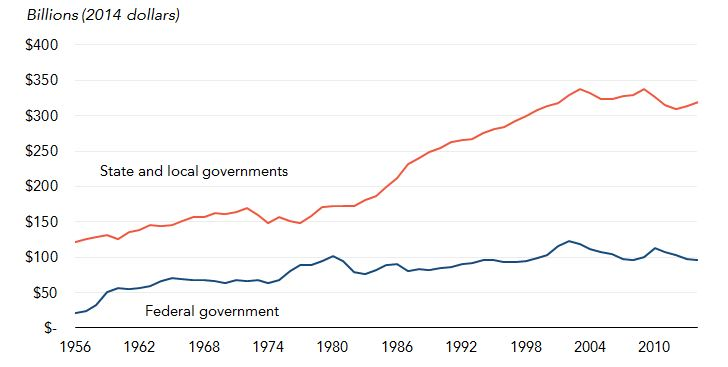
\includegraphics[width=0.8\textwidth]{Chapter-5/Figures/public spending on infrustracture.JPG}}
    \subfigure[]{
        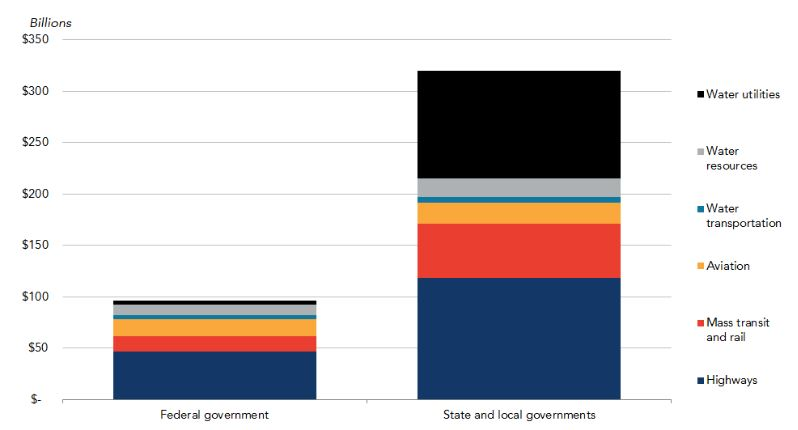
\includegraphics[width=0.8\textwidth]{Chapter-5/Figures/spending on infrastructure.JPG}}
    \caption{Spending of Federal and Subnational Governments on Infrastructure}
    \label{spendingonins}
\end{figure}


\begin{figure}[H]
    \centering
    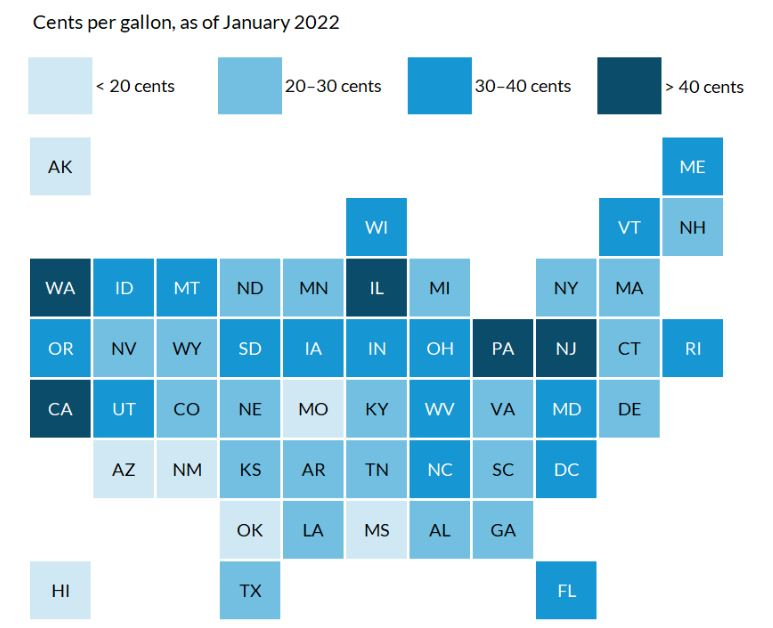
\includegraphics[scale=0.6]{Chapter-5/Figures/fuel tax2.JPG}
    \caption{Gasoline Tax Rate on State Level
        \texttt{} }
    \label{gastax}
\end{figure}




\section{Review and Revisit}
However, some scholars has been arguing that confusion over proper credit assignment allows state lawmakers to claim credit for federal production recently \cite{nicholson2011claiming,bednar2007credit}. In another word, the subnational government can increase their political credit by being a free rider. In this paper, I defined a function to represent Bednar's \cite{bednar2007credit} theory on credit assessment of citizens, which he named as threshold assessment. Threshold assessment means citizens have difficulty in figuring out whether national or subnational government supplied the public goods, they only care if the public goods surpass a specific threshold. This means once the amount surpass the threshold, governments have intention to be a free rider and claim the political credits, thus the subnational governments may welcome the grants from the national government though the grants are restricted.


